\section{Raspberry Pi}
\setauthor{Sebastian Egger}

Das Projekt beinhaltet einen Raspberry Pi 4, welcher als MQTT Broker dient und auf diesem Raspberry Pi läuft auch unser Backend mit DotNet, Docker und Samba.
Der Raspberry Pi hat 4 Gigabyte und eine 32 Gigabyte SSD. 
Die Verbindung zwischen dem Raspberry und der SSD wird mit einem USB-Adapter hergestellt. 
Die SSD wurde unter dem Raspberry mittels einer Platine und Schrauben befestigt. 
Der Raspberry braucht mindestens 0,5 und maximal 0,7 Watt. 
\subsection{Samba}
Unser Raspberry dient als File-Server und zur leichteren Datenübertragung von Windows auf Linux kann man mit Samba von einem Windows Explorer direkt auf den Raspberry Pi zugreifen.
Somit können Files oder Projekte direkt von einem Laptop oder Computer auf den Raspberry PI gelegt werden.

\begin{figure}[H]
    \centering
    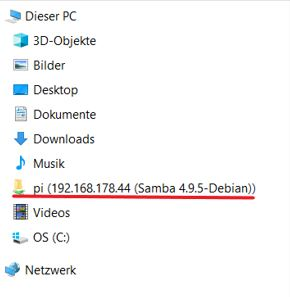
\includegraphics[width=1\textwidth]{pics/RaspberrySamba.JPG}
    \caption{DotNet 6 Nullability von Objekten}
\end{figure}



\subsection {MQTT auf Raspberry Pi:}
Weiteres dient unser Raspberry auch als MQTT-Broker, welcher Messwerte von Sensoren empfängt und an das Backend, welches als MQTT-Client dient, übermittelt. 
Genaueres wie MQTT aufgebaut ist und in welcher Verbindung der MQTT-Broker zu den MQTT-Clients steht wird im Kapitel MQTT beschrieben.

\subsection {Docker auf dem Raspberry Pi installieren und die Verwendung von Docker auf dem Raspberry:}

Docker ist eine Software, welche das Management von Container übernimmt. Ein Container enthält alle Dateien, die zum Ausführen einer Software notwendig sind. 
Die Installation von Docker wird über ein Skript durchgeführt. 
Dieses wird direkt von Docker zur Verfügung gestellt und führt alle Schritte automatisch ohne weitere Eingaben vom Benutzer durch. 
Nach wenigen Minuten ist Docker betriebsbereit. 
Weiter ist auch ein Container mit dem Namen Portainer auf unserem Raspberry Pi installiert, welcher uns eine Liste aller Container und deren Informationen anzeigt.
 


\subsection {Remote Access auf einen Raspberry PI:}
Wenn man auf einen Raspberry PI zugreifen möchte und man hat gerade keinen Monitor zu verfügen , dann kann man mittels SSH von einem Laptop darauf zugreifen.
 Um mittels SSH auf einen Raspberry zugreifen zu können, muss man die Ip-Adresse in einem Netzwerk von dem Raspberry wissen. 
 Falls man eine FRITZ!Box als WLAN-Router nutzt, kann man sich über die Ip-Adresse (192.168.178.1) im Browser auf seiner FRITZ!Box und eine Übersicht der verbundenen Geräte anzeigen lassen, wo auch unter anderem der Raspberry PI connected ist. 

 \subsection{Was sind Ip-Adressen:}
Im oberen Kapitel Remote Access ist oft das Wort Ip-Adresse gefallen, deswegen wird in diesem Unterpunkt eine kleine Einführung was Ip-Adressen sind und wofür sie gebraucht werden. 
Eine Ip-Adresse ist eine Adresse in Computernetzen, welche von dem Router vergeben wird.
 Einem Gerät kann maximal eine Ip-Adresse zugewiesen werden, jedoch kann die Ip-Adresse auch wechseln, wenn sich das Gerät zum Router erneut verbindet. 
 Im Router gibt es aber auch die Funktion, dass ein Gerät immer eine bestimmte Ip-Adresse zugewiesen bekommt. 






\section{MQTT}
\setauthor{Sebastian Egger}

\subsection{Was ist MQTT:}
MQTT ausgeschrieben Message Queuing  Telemetry Transport ist ein Protokoll, welches Nachrichten von einer Maschine zu einer anderen Maschine schickt. 
Ein MQTT Netzwerk besteht  aus mindestens einen MQTT-Broker und zwei MQTT-Clients. 
Wenn ein MQTT-Client eine Message an einen anderen MQTT-Client senden will, sendet er als erstes eine Message zu dem MQTT-Broker, welcher die Message zu einem sogenannten Topic zuweist.
Ein Topic ist ein Bereich, wo bestimmte Nachrichten aufgelistet werden. 
Ein Topic in unserem Fall lautet mqtt/noice für den Noice-Sensor.  
Wenn ein oder mehrere MQTT-Clients diese Nachricht empfangen wollen, dann subscriben diese auf das Topic. 
Durch das subscriben von den Clients werden diese, sobald eine neue Message an das Topic gesendet wurde, benachrichtigt und können diese nun empfangen. 

\subsection {Verwendung von MQTT in unserem Projekt:}
Unser Projekt besteht aus 2 MQTT-Clients und 1 MQTT-Broker. 
Zu einem ist die Sensor Box ein MQTT-Client, welcher die Messwerte an den MQTT-Broker sendet. 
Der MQTT-Broker ist in unserem Projekt der Raspberry PI. 
Zum Empfangen der Daten liest unser Backend, welcher der zweite MQTT-Client ist, die Daten vom Raspberry ein.

\subsection{MQTT-Explorer:}
MQTT-Explorer ist eine kostenlose Software, welches sich für das Testen einer Connection zwischen MQTT-Client und Broker bestens eignet.
Der MQTT-Explorer ist ein weiterer MQTT-Client.
Als erstes loggt man sich mit der Ip-Adresse und Port des Brokers sowie den dazugehörigen Username und Password ein.

\begin{figure}[H]
    \centering
    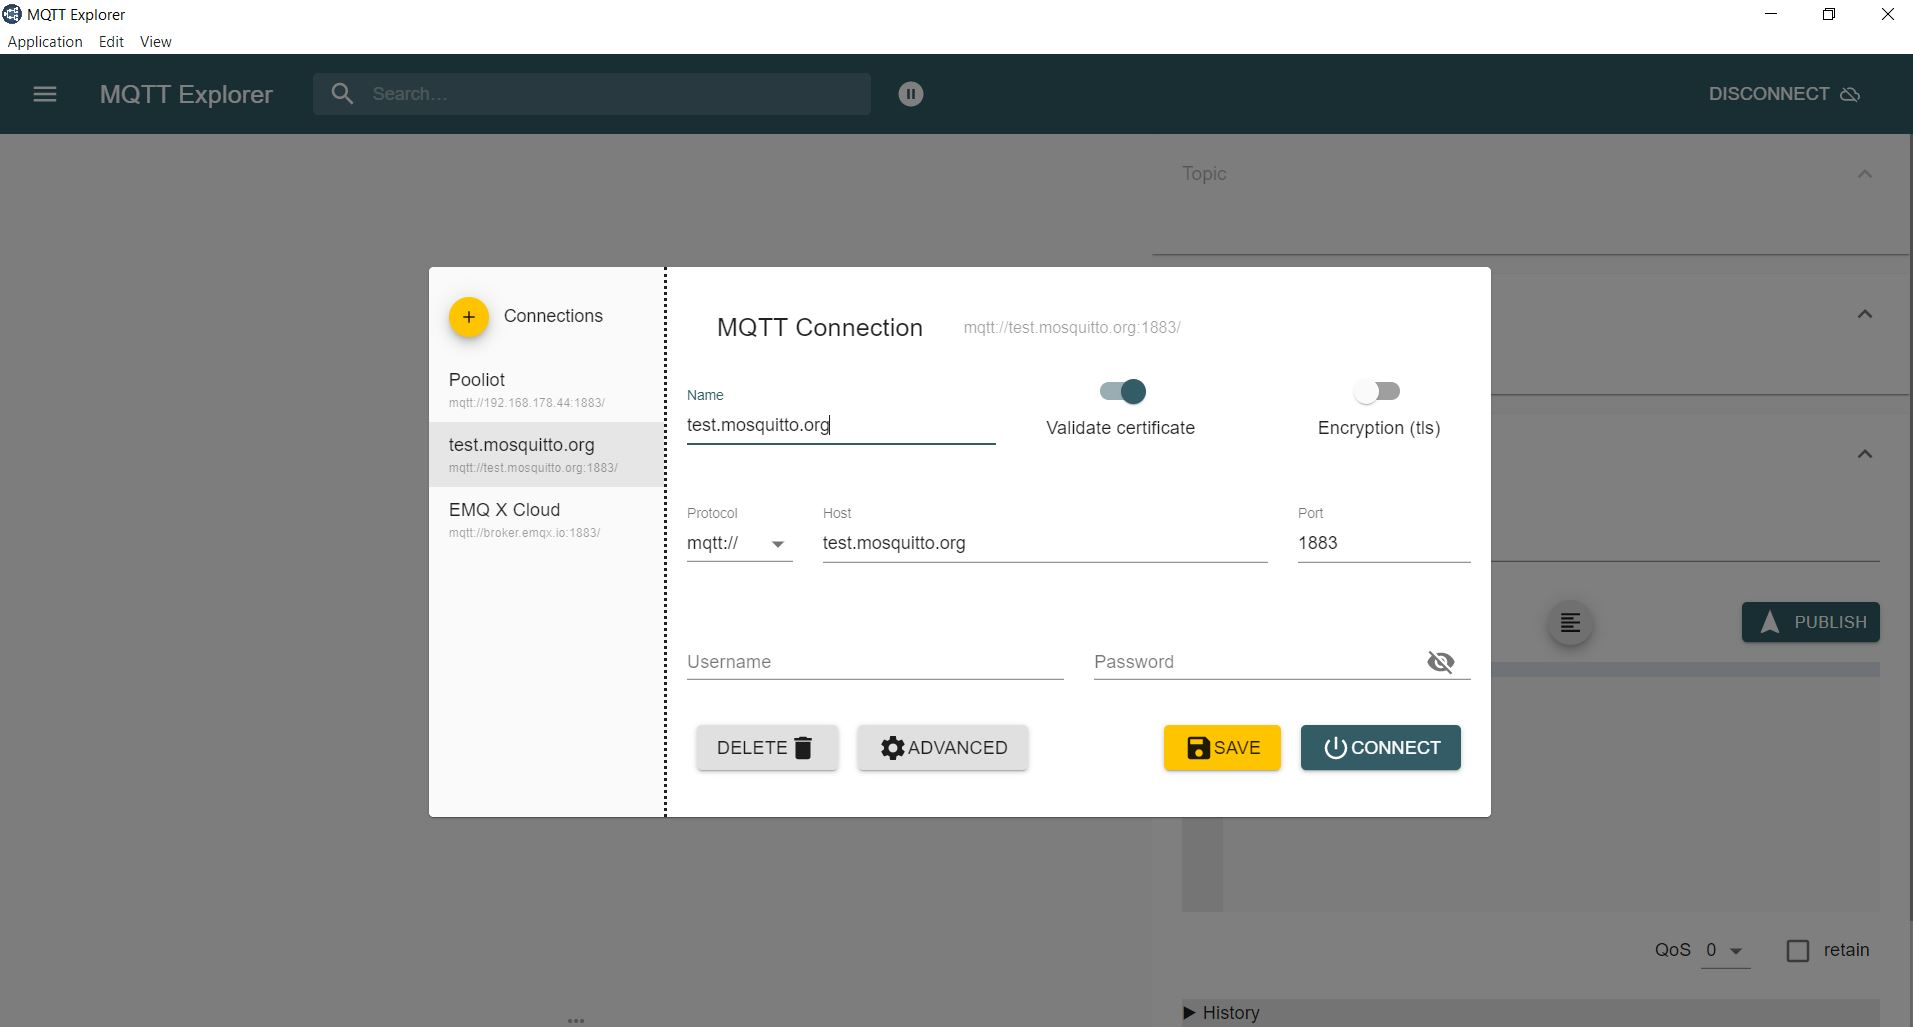
\includegraphics[width=1\textwidth]{pics/MQTTExplorerStartScreen.JPG}
    \caption{DotNet 6 Nullability von Objekten}
\end{figure}


 Wenn eine Verbindung zu einem MQTT-Broker möglich ist, wird ein Screen mit dem Namen des Brokers und den dazugehörigen Topics aufgelistet. 
 In diesem Foto wurde sich für eine grafische Abbildung mit dem MQTT-Broker test.mosquitto.org verbunden.  

 \begin{figure}[H]
    \centering
    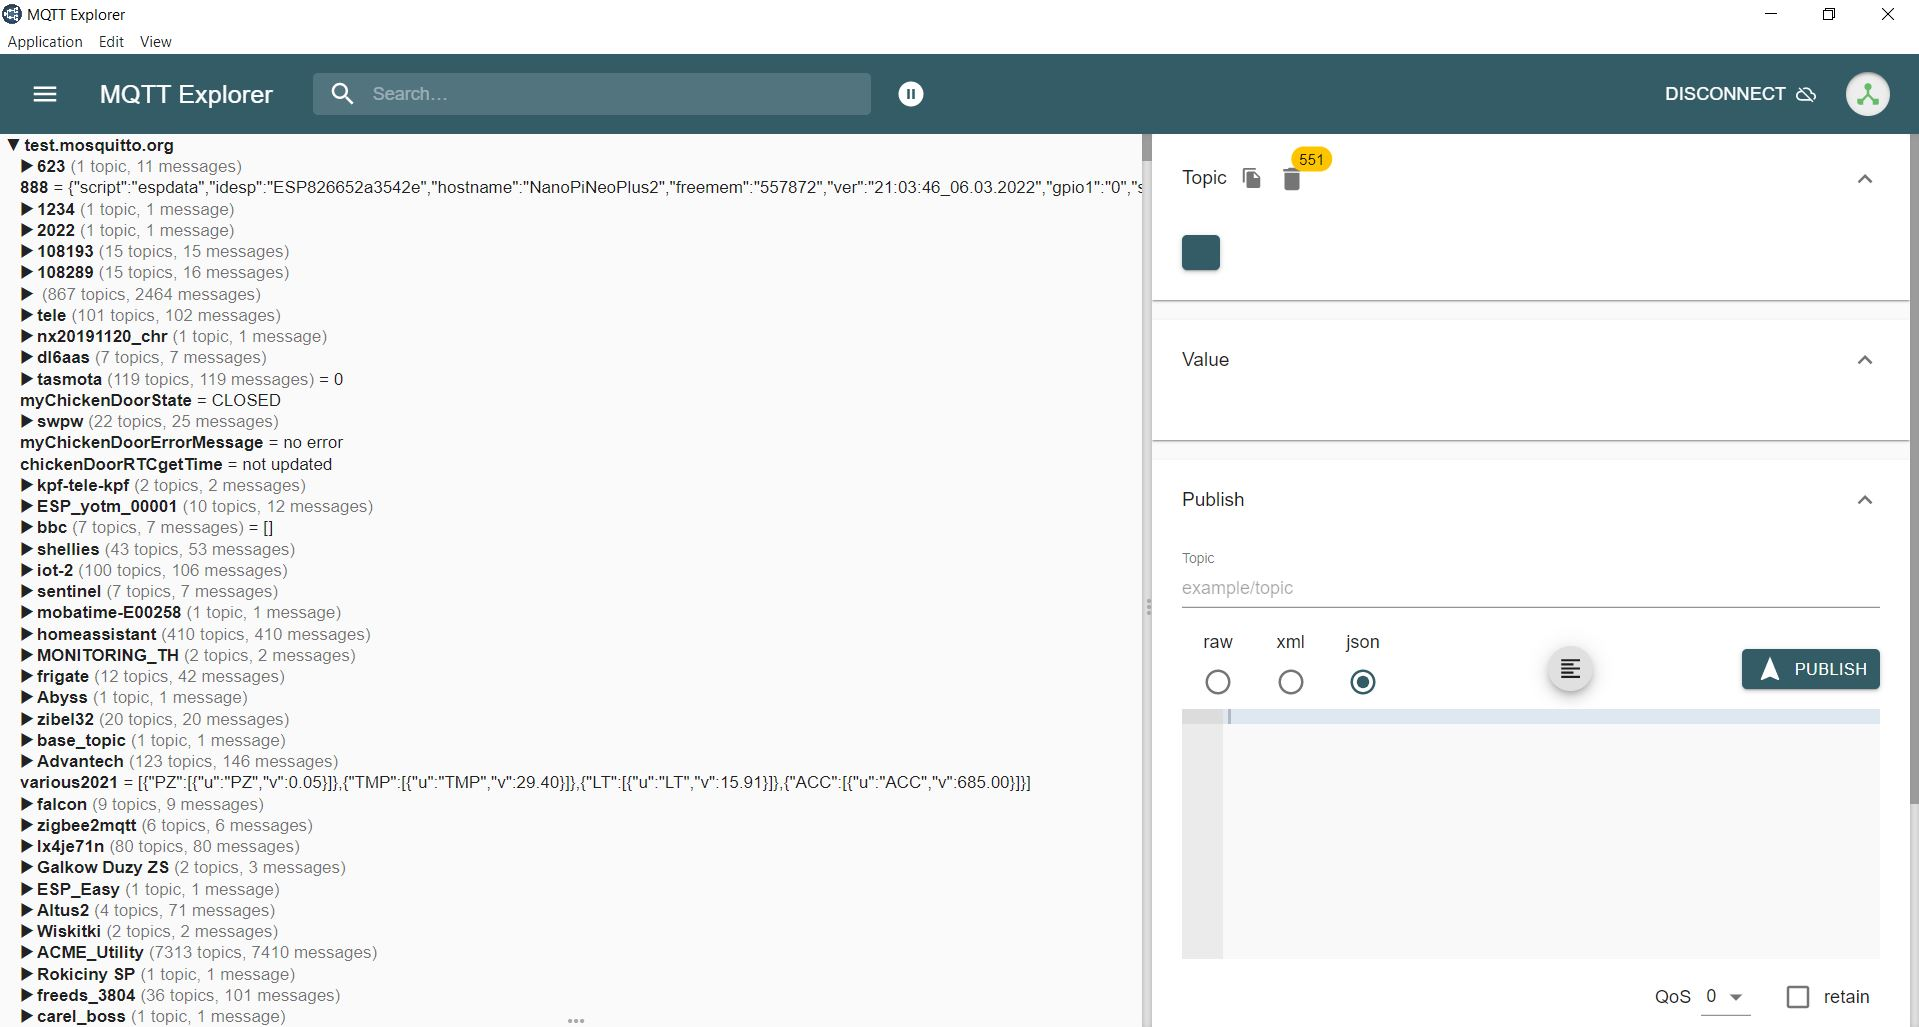
\includegraphics[width=1\textwidth]{pics/MQTTExplorerTestDemo.JPG}
    \caption{DotNet 6 Nullability von Objekten}
\end{figure}








\section{.Net}
\setauthor{Sebastian Egger}

\subsection {Backend Projekte}



Das Backend setzt sich aus 12 Projekten zusammen, welche in C\# .Net 5 geschrieben sind.

\begin{itemize}
    \item CommonBase
\end{itemize}

In CommonBase befinden Klassen und Methoden, die wiederverwendbar sind um Code verdoppelung zu vermeiden.

\begin{itemize}
    \item CSharpCodeGenerator.Logic
\end{itemize}

CSharpCodeGenerator.Logic dient zum automatischen generieren von den Entitäten 
in SnQPoolIot.Logic, SnQPoolIot.WebApi und SnQPoolIot.AspMvc.
In SnQPoolIot.Contracts werden Entitäten als Interfaces angegeben.
Wenn danach die Solution gebuildet wird, werden für die Entitäten Klassen und die dazugehörigen Controller angelegt.
Es werden auch Beziehung und Keys zwischen den Entitäten generiert.


\begin{itemize}
    \item SnQPoolIot.Adapters
\end{itemize}

SnQPoolIot.Adapters bietet uns einen direkten Zugriff auf die Logic.
Der Zugriff auf die Logic kann dadurch entweder direkt erfolgen oder per Rest über die WebApi.

\begin{itemize}
    \item SnQPoolIot.WebApi
\end{itemize}

Der Zugriff auf die Messwerte wird durch Rest-Zugriffe in SnQPoolIot.WebApi providet.
Auf die Daten kann aber nur zugegriffen werden, wenn man sicher vorher mit einem Account einloggt.  

\begin{itemize}
    \item SnQPoolIot.Contracts
\end{itemize}

SnQPoolIot.Contracts beinhaltet alle notwendigen Schnittstellen und Enumerationen des Projektes.
Hier werden die Entitäten als Interfaces angelegt, 
welche von CSharpCodeGenerator.Logic als Klassen und Controller in den oben genanten Projekten generieren.

\begin{itemize}
    \item SnQPoolIot.Logic
\end{itemize}

SnQPoolIot.Logic ist das Kernstück des Projektes. 
Durch die Logic können wir alle Daten von der Datenbank holen. 
Die Datenbank auf welche die Logik zugreift ist eine Sqlite Datenbank und der Zugriff und das erzeugen der Datenbank wird mittels Entityframework.Sqlite durchgeführt.

\begin{itemize}
    \item SnQPoolIot.Transfer
\end{itemize}

SnQPoolIot.Transfer verwaltet die Transferobjekte für den Datenaustausch zwischen den Layers.

\begin{itemize}
    \item SnQPoolIot.AspMvc
\end{itemize}

SnQPoolIot.AspMvc ist ein Ersatz für das Frontend.
Hier werden die Funktionen wie zum Beispiel einloggen eines Users oder anzeigen von Messwerten dargestellt.

\begin{itemize}
    \item SnQPoolIot.ConApp
\end{itemize}

In SnQPoolIot.ConApp werden User mit verschiedenen Rechten angelegt, die für die Authentifizierung benötigt werden.

\subsection {DotNet 5 vs DotNet 6}

Unser Backend wurde wie oben bereits erwähnt mit DotNet 5 geschrieben, weil die Umstellung zu DotNet 6 einiges mit sich bringt.
Der Hauptgrund warum wir uns für DotNet 5 entschieden haben, ist die Unterscheidung der Nullability von Objekten und die dadurch ausgelösten Warnings.
In DotNet 5 werden durch Objekte die Null sein könnten keine Warnings angezeigt und man ersparrt sich etliche Zeit, wenn man sich nicht durch die Warnings käpfen muss.

\begin{figure}[H]
    \centering
    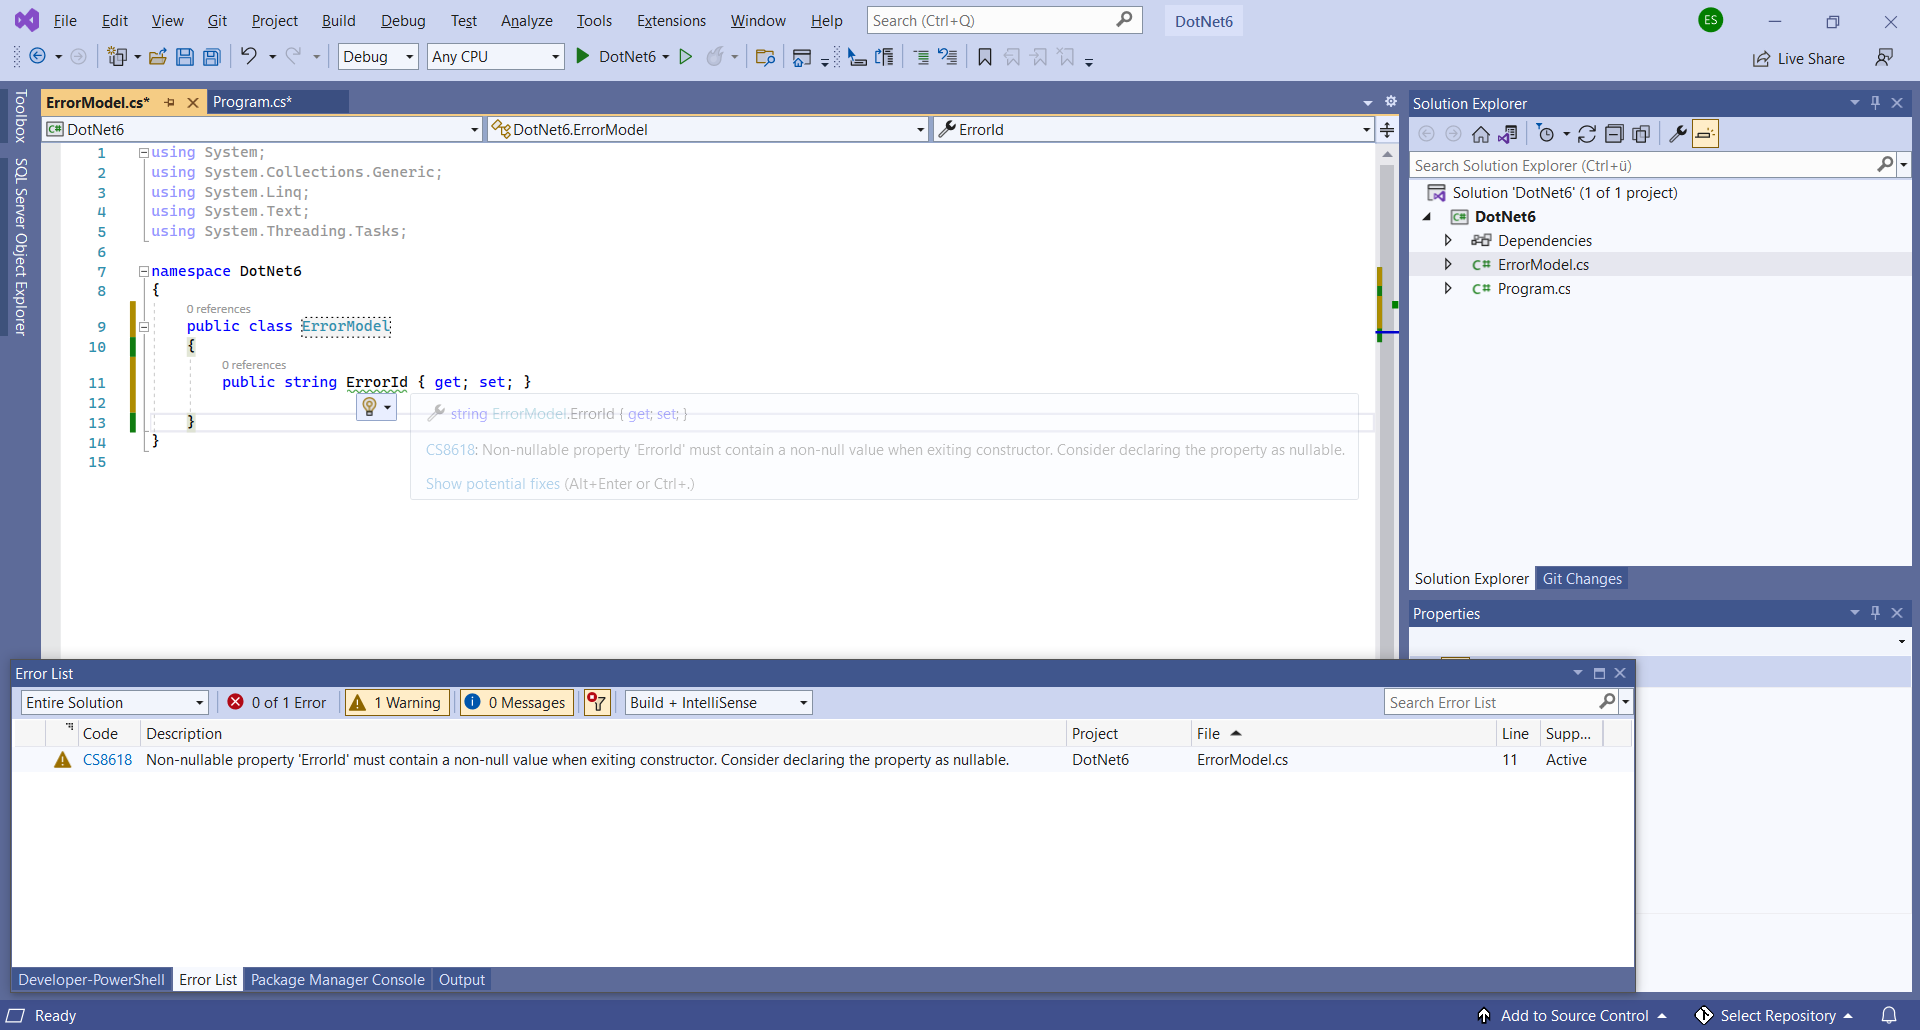
\includegraphics[width=1\textwidth]{pics/DotNet6Nullability.png}
    \caption{DotNet 6 Nullability von Objekten}
\end{figure}


\begin{figure}[H]
    \centering
    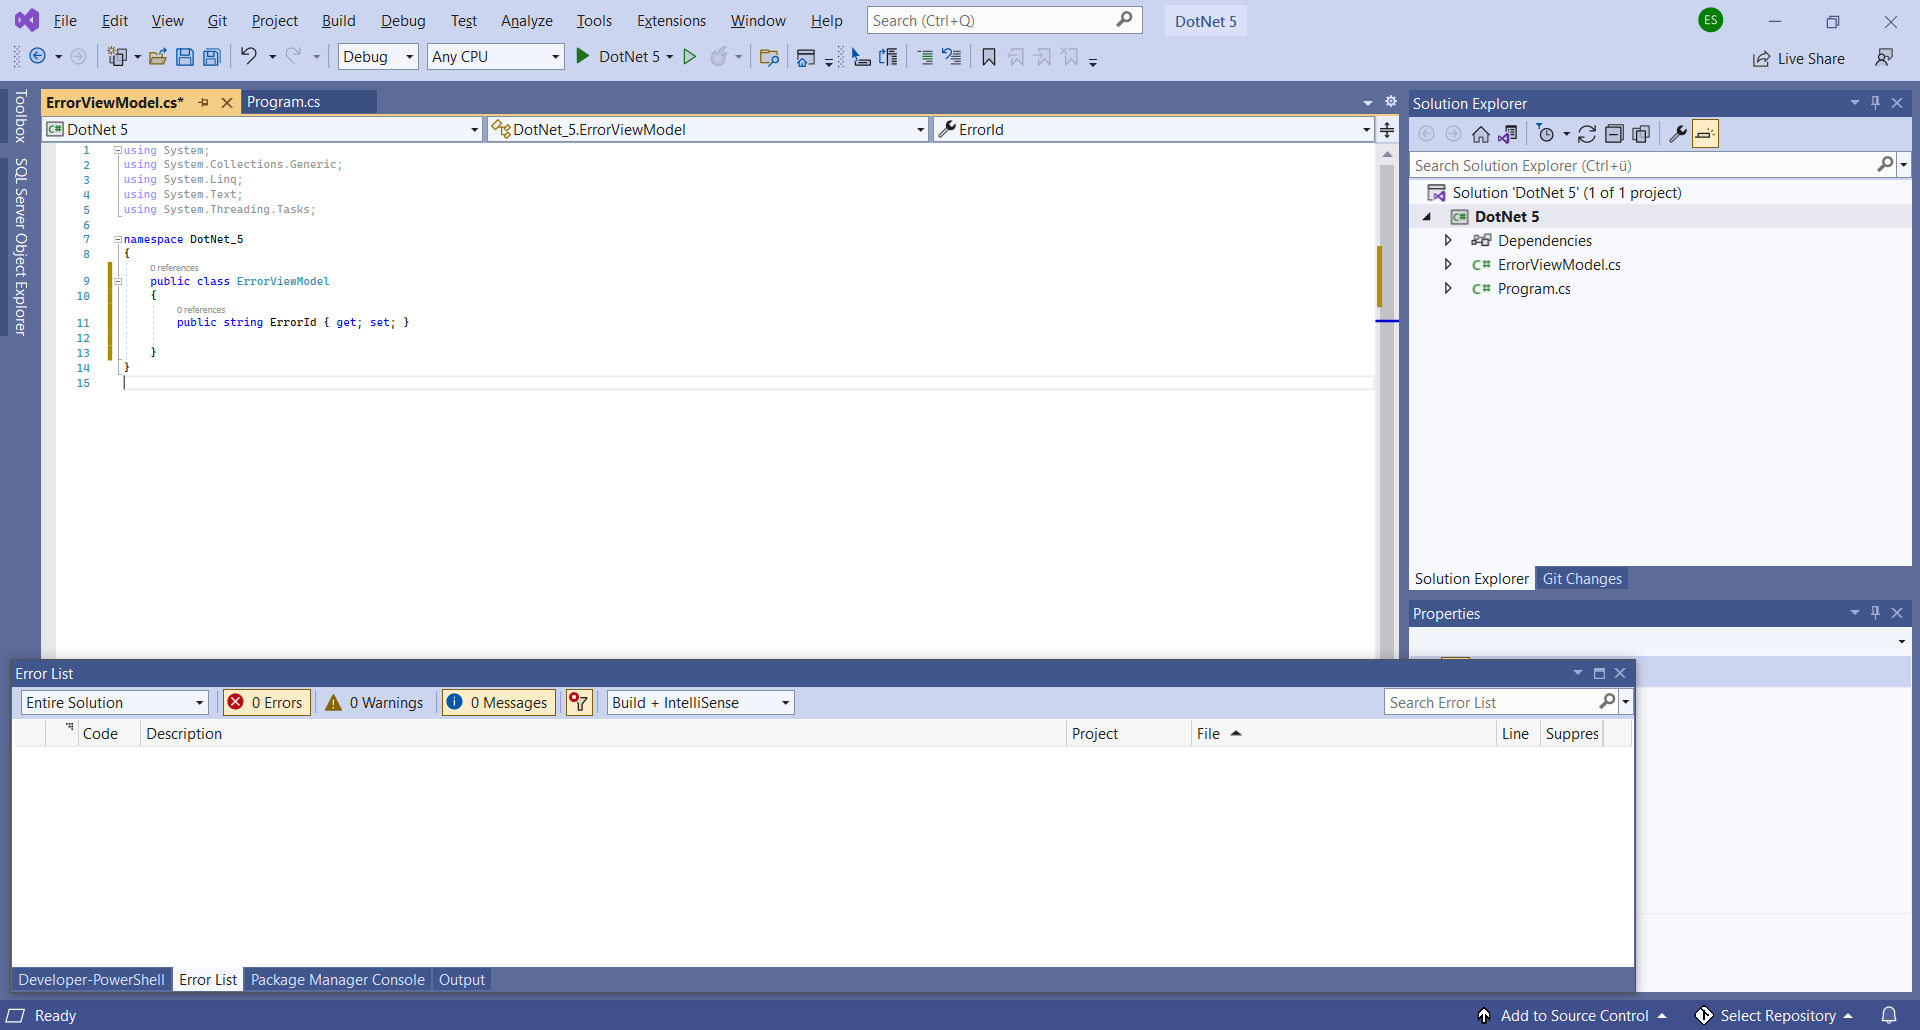
\includegraphics[width=1\textwidth]{pics/DotNet5Nullability.png}
    \caption{DotNet 5 keine Warnungs durch Nullability}
\end{figure}




Jedoch im Vergleich zu DotNet 5 hat DotNet 6 eine bessere Leistung, denn bei einer Ausführung in der Cloud sinkt es die Computekosten, welches ich als riesigen Vorteil sehe.
Einen weiteren Nachteil finde ich ist die Lesbarkeit des Codes.

Hier ein Beispiel zu diesem Thema:

Hier sieht man eine Consolen Apllication in DotNet 6 und man kann sehen,
dass es keine Übersicht gibt wie man anfängt. Eine Person welche zum ersten Mal ein Tutorial, welches in DotNet 5 beschrieben wurde, nachprogrammiert, hat keine Ahnung 
wo man in DotNet 6 die Usings oder die Methoden implementiert. 




\begin{figure}[H]
    \centering
    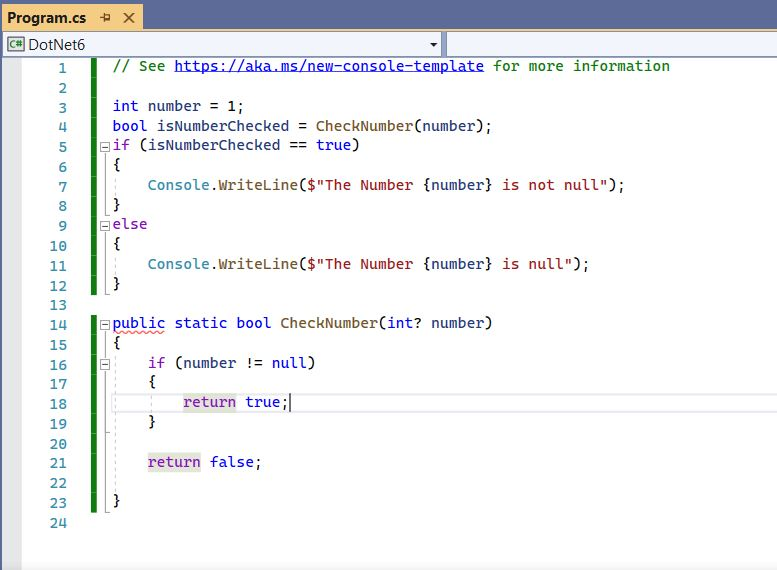
\includegraphics[width=1\textwidth]{./pics/DotNet6ConApp.JPG}
    \caption{DotNet6ConApp}
\end{figure}


\begin{figure}[H]
    \centering
    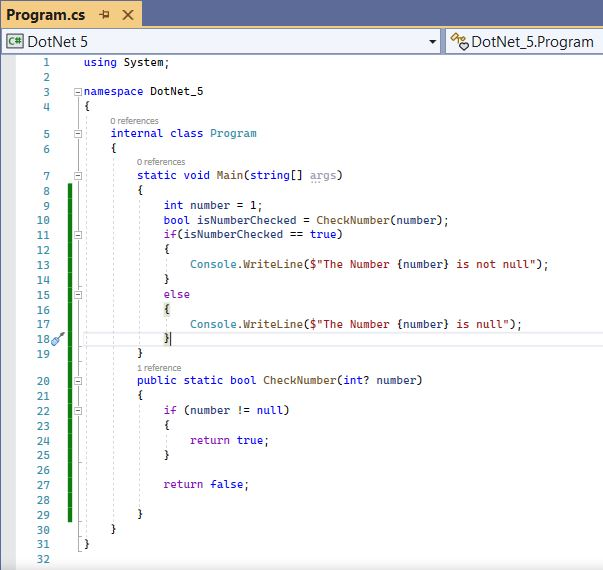
\includegraphics[width=1\textwidth]{./pics/DotNet5ConApp.JPG}
    \caption{DotNet5ConApp}
\end{figure}


Im Vergleich zu DotNet 6 kann man hier klar erkennen, wo man die Usings und die Methoden hinschreibt.




Warum Sqlite und nicht SqlServer als Datenbank:

In unserem Projekt verwenden wir Sqlite als Datenbank, weil die Datenbank ansonsten nicht auf dem Raspberry Pi laufen würde.
Unser Raspberry Pi verwendet Linux als Betriebssystem und Microsoft meint, dass ein SqlServer nicht für Linux geeignet sind und deshalb gibt es keinen SqlServer für Raspberry Pi's.
Weiteres, wenn es einen SqlServer für den Raspberry Pi geben würde, wird wegen dem Speicherplatz noch immer eine Sqlite Datenbank einen großen Vorteil anbieten.






